%%%% necessary customization for the appendix and headers
\appendix 
\makeatletter
\addtocontents{toc}{\protect\renewcommand\protect\cftchappresnum{\@chapapp\ }}
\makeatother
\renewcommand{\thechapter}{\Alph{chapter}}

\chapter{Chapter 3 Appendix} \label{chap:appendix-3}

%% add your chapter text here
\section{Annotation Instructions}
\label{sec:annotation-instructions}
\subsection{Questions}
\textbf{Question 1 – Which document do you prefer?}
In this question, you are asked to choose which document version you prefer. Some examples of qualities you may use to decide your preference include: 
\begin{itemize}
    \item The quality of the content – The text is grammatical and understandable. E.g. Document A contains major grammatical errors while Document B only contains minor errors.
    \item The formatting – The formatting is reasonable and matches the formatting of the intended document type. E.g. A poster contains panels and each panel contains a header and body text.
    \item The style – The document matches the style of the intended document type. E.g. Shorter, bulleted sentences in a slide deck.
    \item Information represented in the document – The document contains sufficient information to represent the input document. E.g. A blog post represents the most important sections from the input document.
\end{itemize}


The above criteria are non-exhaustive. Not all criteria must be met, and you may use other relevant criteria to make your decision. 
You are not rating the document for factual correctness,\footnote{The annotators are non-experts and do not have the background to determine factual correctness of scientific information. Instead, they are encouraged to use the original paper to understand if the information presented in the documents represent the information in the paper, to the best of their understanding.} and only need to refer to the corresponding scientific article if it will aid in making your preference. 
You can answer this question with either Document A or Document B.


\textbf{Question 2 – On a scale of 1-3, to what degree do you prefer your selection?
}

\noindent In this question you will rate the degree to which you prefer your selection, on the following scale:
\begin{enumerate}
    \item Small preference – The documents are similar in quality and only contain minor differences that affect my preference.
    \item Moderate preference – I clearly prefer one document but the differences are not major.
    \item Strong preference – I have a strong preference for one document and the differences between the documents are major.
\end{enumerate}

\textbf{Question 3 – Why do you prefer your selection? (You may select more than one property)}
\begin{itemize}
    \item[$\square$] Formatting
    \item[$\square$] Information
    \item[$\square$] Quality
    \item[$\square$] Style
    \item[$\square$] Other (free text)
\end{itemize}


\subsection{Edge cases}
For most edge cases, it is up to your discretion on how to best handle the case. However, below are a few examples of how you could consider certain edge cases:

\textbf{Example 1: Slides 1-5 of Document A are higher quality but slides 6-10 of Document B are higher quality.
}
You could reason that the first slides represent the most important information, and choose Document A. However, since Document B contained higher quality slides for another portion of the document, you could rate your degree of preference as “Small preference.”

\textbf{Example 2: Document A more closely matches the style of the intended document type, but Document B contains more relevant information to the source document.
}
You could consider if Document A contains sufficient information to represent the input document, such as representing the most important sections. If yes, then you could prefer Document A. If not, then you could reason that information content is more important than style, and prefer Document B.

\textbf{Example 3: Document A contains more relevant information than Document B, but also contains major formatting errors, such as text being cut off from the document.}

You could reason that although Document A contains more relevant information, the major formatting errors are significant enough to prefer Document B.

\textbf{Example 4: Neither document matches the style or formatting of the intended document type. 
}
Since neither document matches the style or formatting of the intended document type, you could consider other criteria, such as quality of content or the information represented. 


\input{research-chapters/3-chapter/tables/tmp_results}
\section{Temperature Experiments}\label{sec:temp-exp}
We experiment with the temperature of the generations to see how temperature affects performance. We randomly sample 100 documents each from LongSumm and Doc2PPT for the blog and poster generation tasks, respectively. We use the entirety of the Paper-Poster dataset, since it contains less than 100 examples. We use \texttt{gpt35-16k} and experiment with the temperatures $[0.0, 0.25, 0.5, 0.75, 1.0]$. The results of this experiment can be found in Table~\ref{tbl:temp-exp}. As we can see from the results, there seems to be little consistency across the different types in which temperature performs the best.  



\section{Longsumm Blind Test Set Results}\label{sec:longsumm-blind}
We submit the final documents from GPT4, the best performing model overall, to the Longsumm blind test set evaluation. We compare the documents generated with and without the intermediate step. We see that without the intermediate representation we get a Rouge-1 score of 46.8 while the results generated without the intermediate representation received a Rouge-1 score of 46.4. We note that this blind test set of 22 papers is significantly smaller than the evaluation data (505 papers) we used in the main body of this paper. Despite not designing a task specific method, we place second on the leaderboard, showing the powerful capabilities of LLMs in long document generation.

\section{Example Outputs}\label{sec:example-outputs}
We provide examples of the outputs generated with and without the intermediate representation below. The documents in all examples are generated with GPT4 ($\texttt{gpt4-32k}$). Figure~\ref{fig:ex-slides} includes example slide generations, Figure~\ref{fig:ex-blogs} includes example blog generations, and Figure~\ref{fig:ex-posters} includes example poster generations. 

\begin{figure*}[t!]
    \centering
    \begin{subfigure}[t]{0.5\textwidth}
        \centering
        \frame{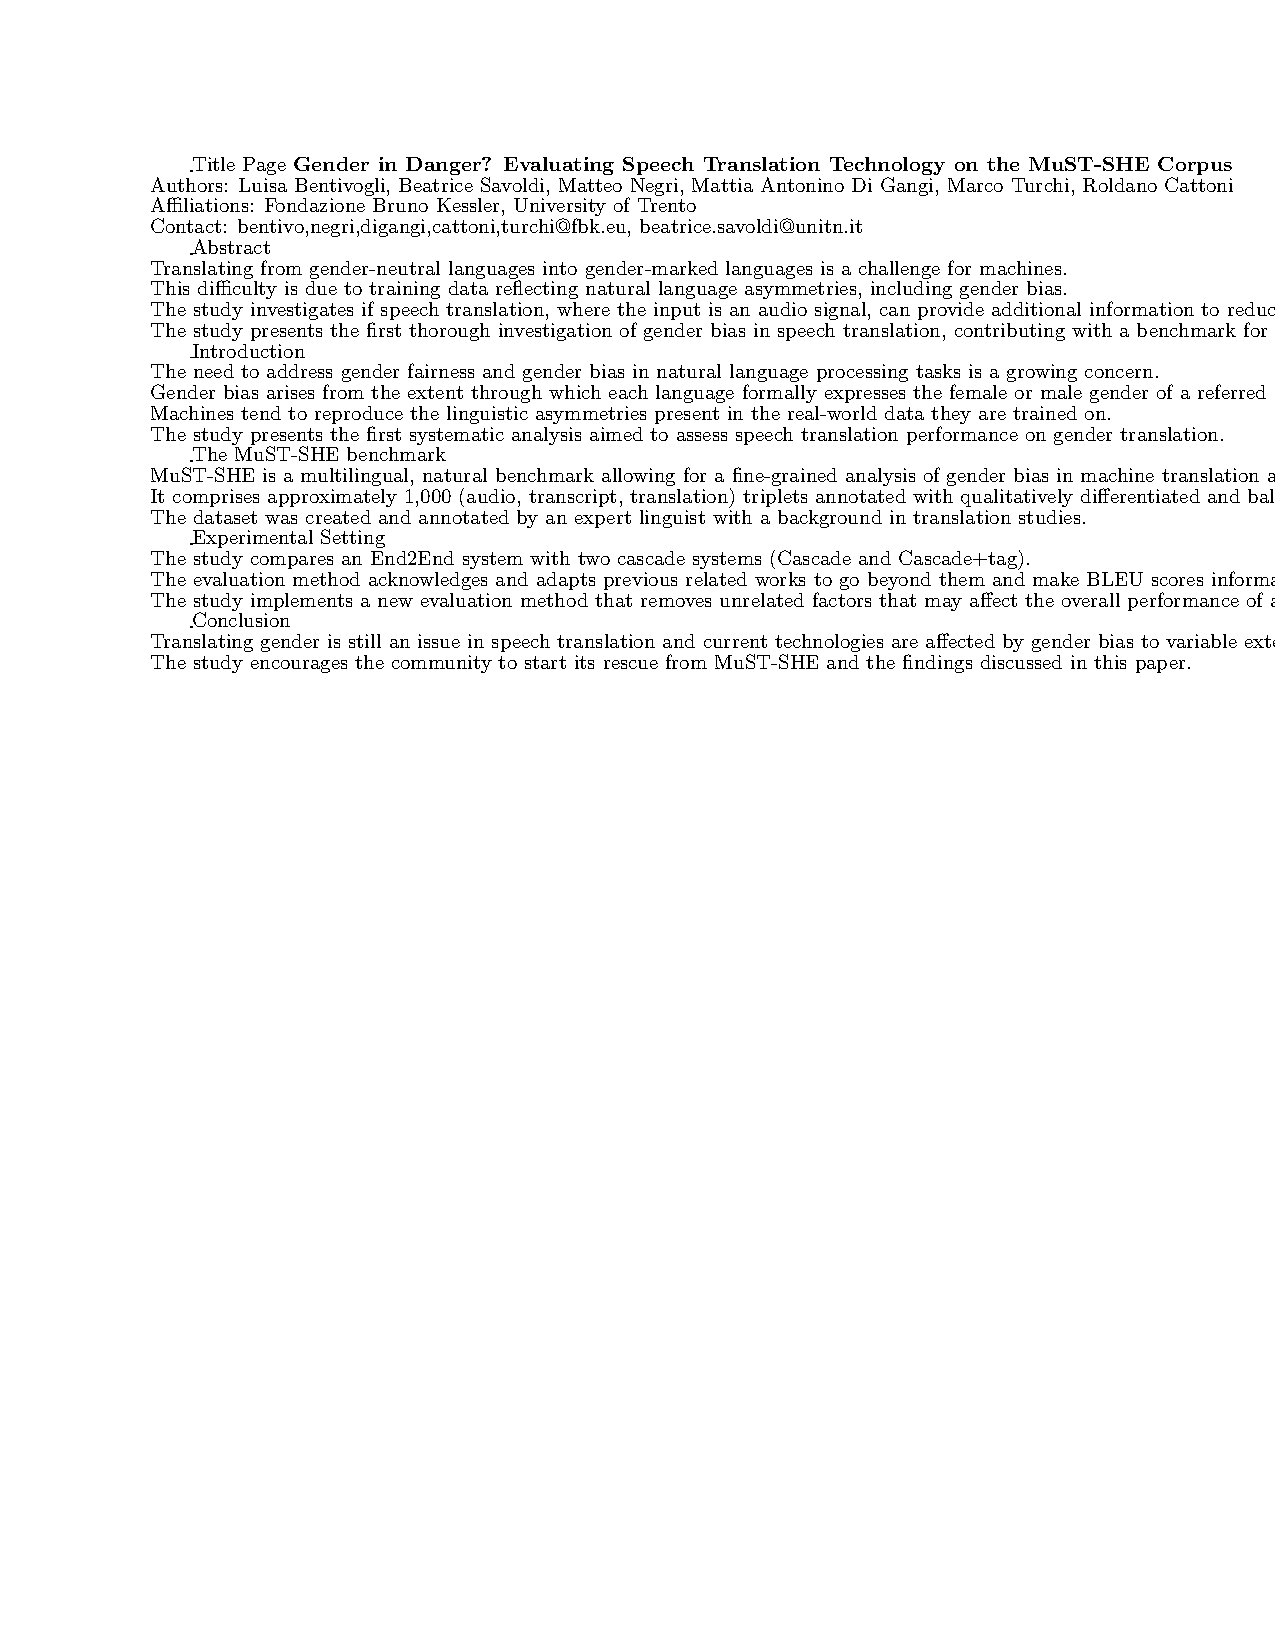
\includegraphics[width=.95\textwidth]{research-chapters/3-chapter/images/ex-slide-skiprep.pdf}}
        \caption{Document generated without intermediate representation. This example is not cropped.}
    \end{subfigure}%
    ~ 
    \begin{subfigure}[t]{0.5\textwidth}
        \centering
        \frame{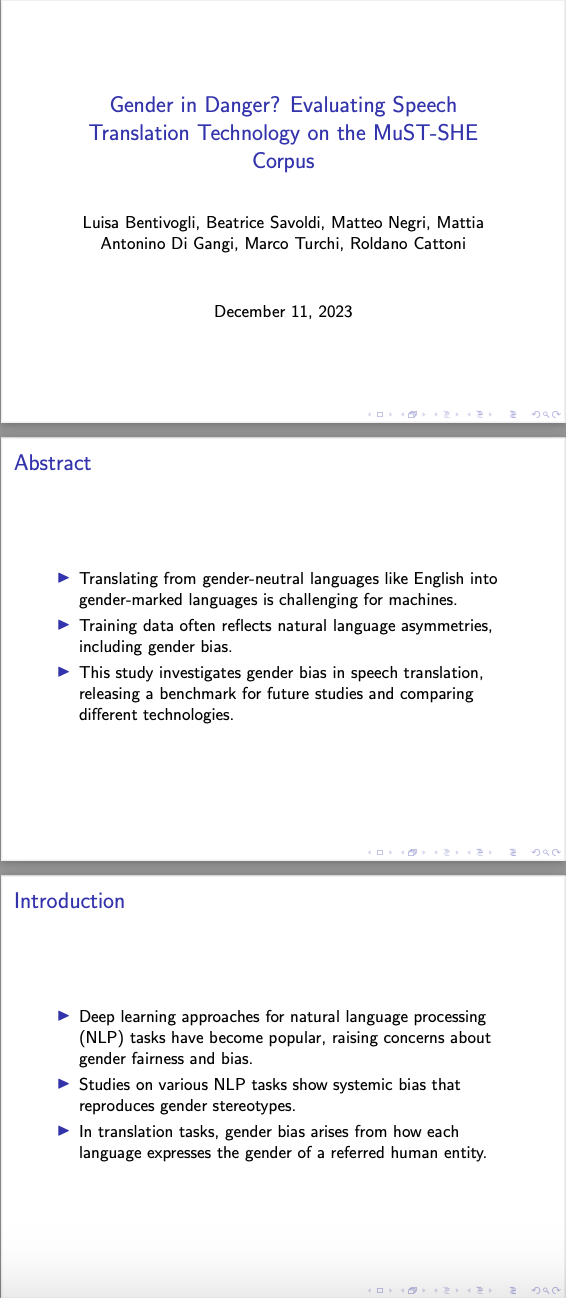
\includegraphics[width=.9\textwidth]{research-chapters/3-chapter/images/ex-slide-withrep.png}}
        \caption{Document generated with intermediate representation. This example is cropped for space and includes an additional 4 slides that are not included for space.}
    \end{subfigure}
    \caption{The above documents are example slides generated by GPT4 ($\texttt{gpt4-32k}$) with and without the intermediate representation. We can see that without the intermediate step, the model did not generate a true slide deck.}
    \label{fig:ex-slides}
\end{figure*}

\begin{figure*}[t!]
    \centering
    \begin{subfigure}[t]{0.45\textwidth}
        \centering
        \frame{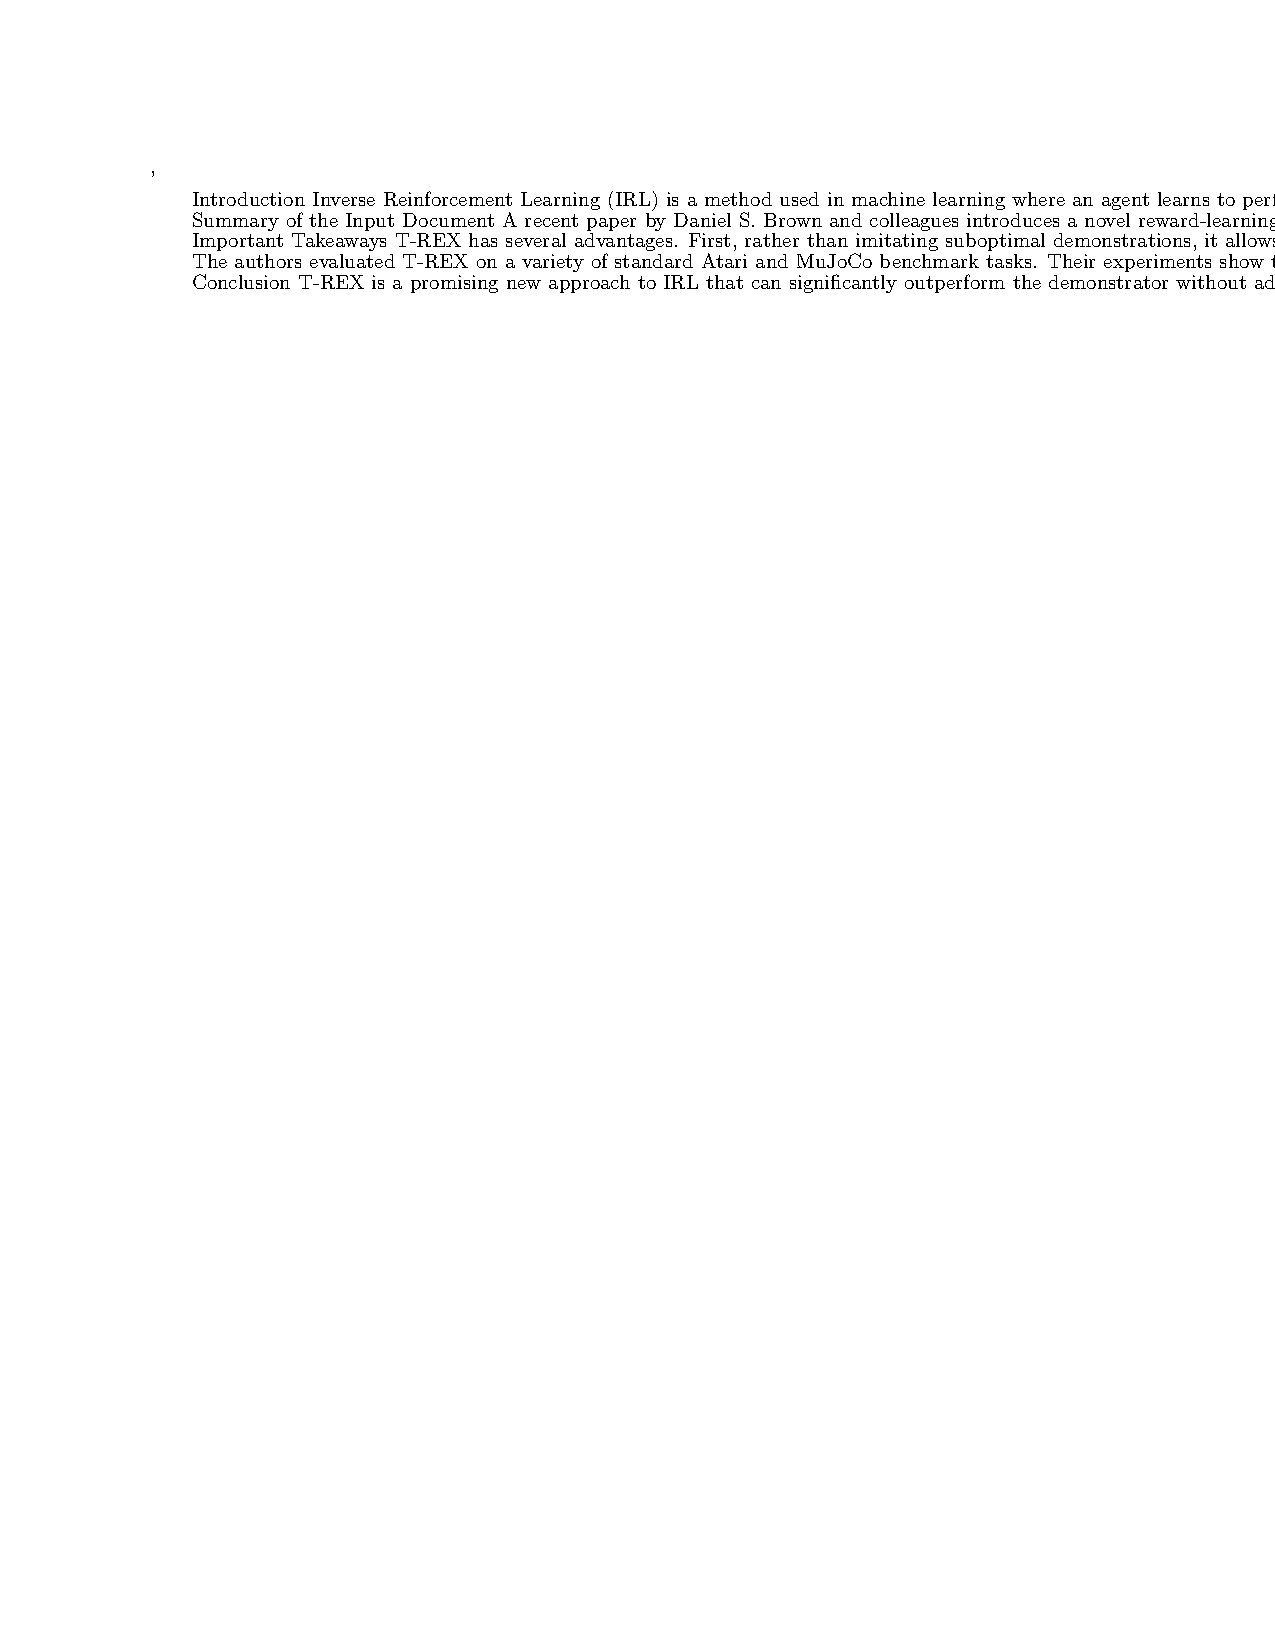
\includegraphics[width=.95\textwidth]{research-chapters/3-chapter/images/ex-blog-skiprep.pdf}}
        \caption{Document generated without the intermediate representation. This example is not cropped.}
    \end{subfigure}%
    ~ 
    \begin{subfigure}[t]{0.45\textwidth}
        \centering
        \frame{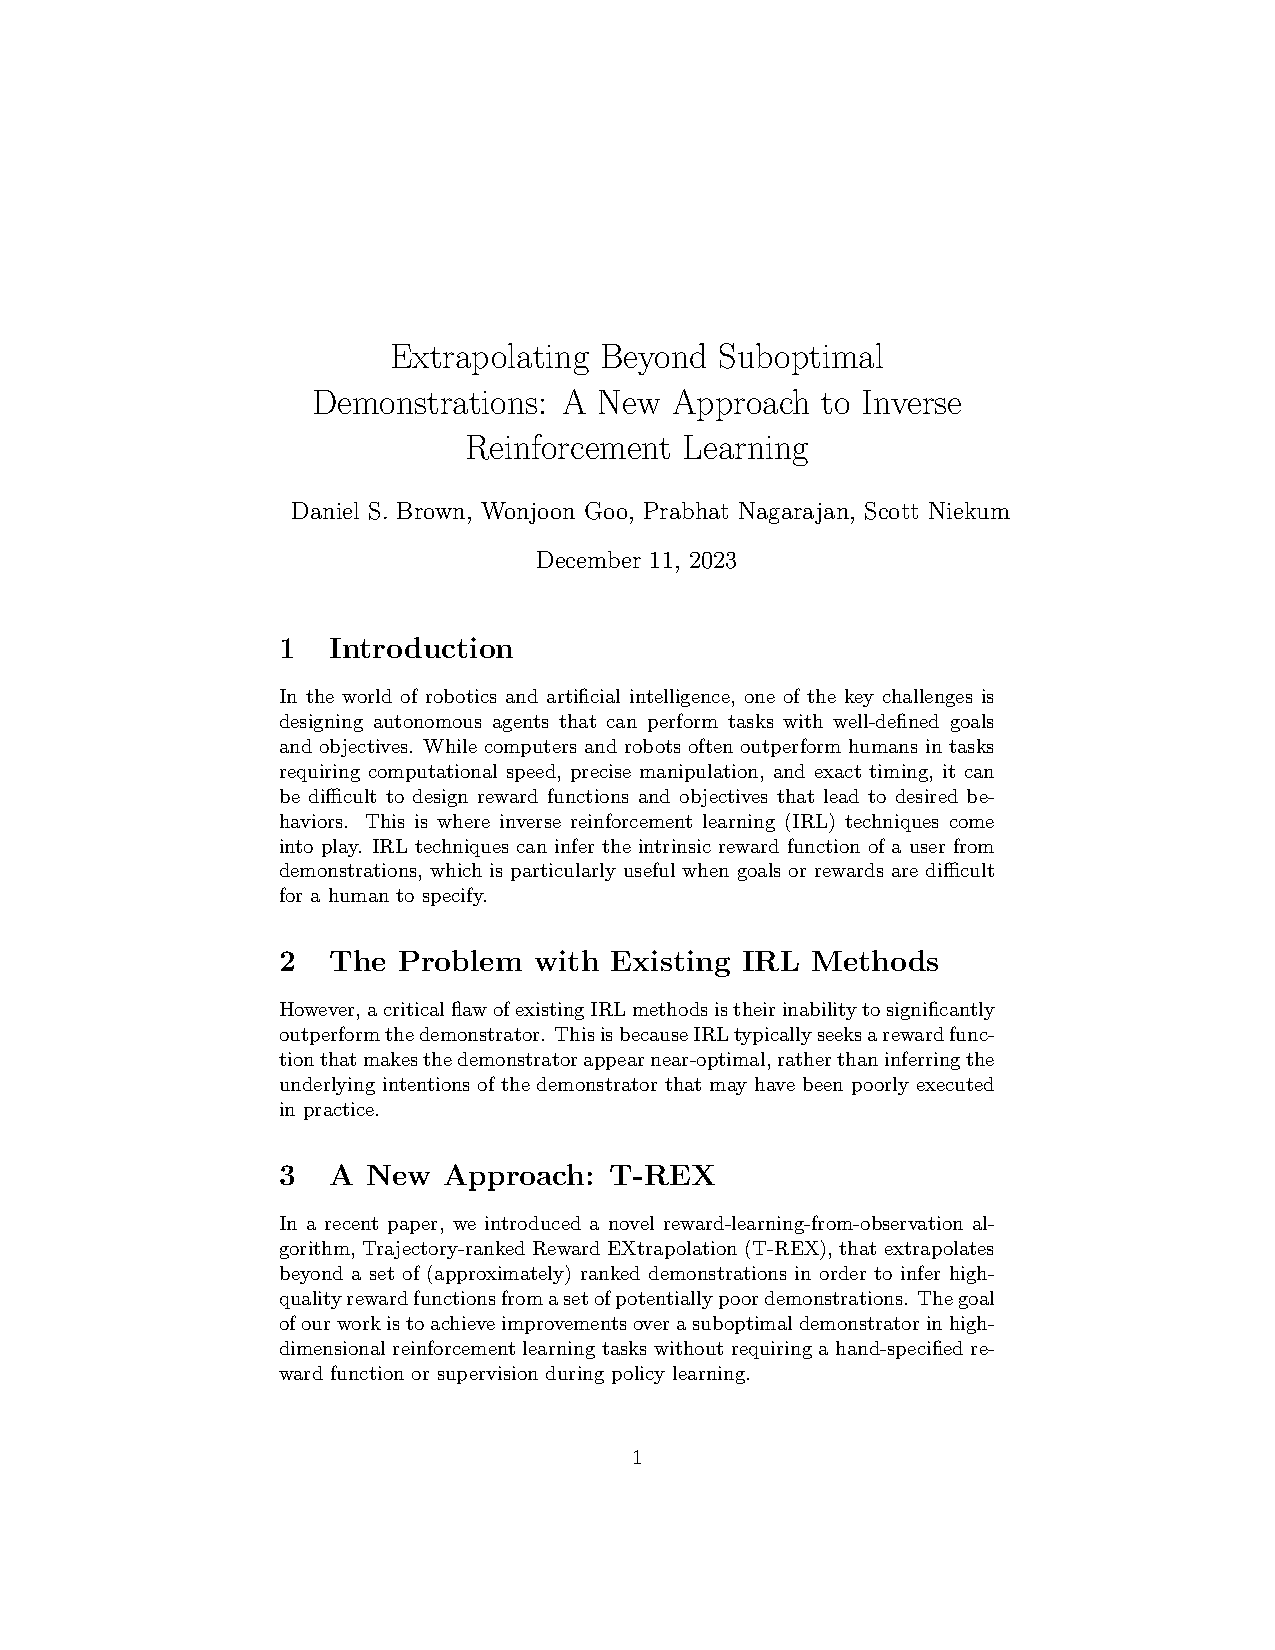
\includegraphics[width=.95\textwidth]{research-chapters/3-chapter/images/ex-blog-withrep.pdf}}
        \caption{Document generated with the intermediate representation. This example is cropped for space and includes an additional page of text.}
    \end{subfigure}
    \caption{The above documents are example blog posts generated by GPT4 ($\texttt{gpt4-32k}$) with and without the intermediate representation. We can see that without the intermediate representation, the model did not properly format the LaTeX file for compilation.}
    \label{fig:ex-blogs}
\end{figure*}

\begin{figure*}[t!]
    \centering
    \begin{subfigure}[t]{0.45\textwidth}
        \centering
        \frame{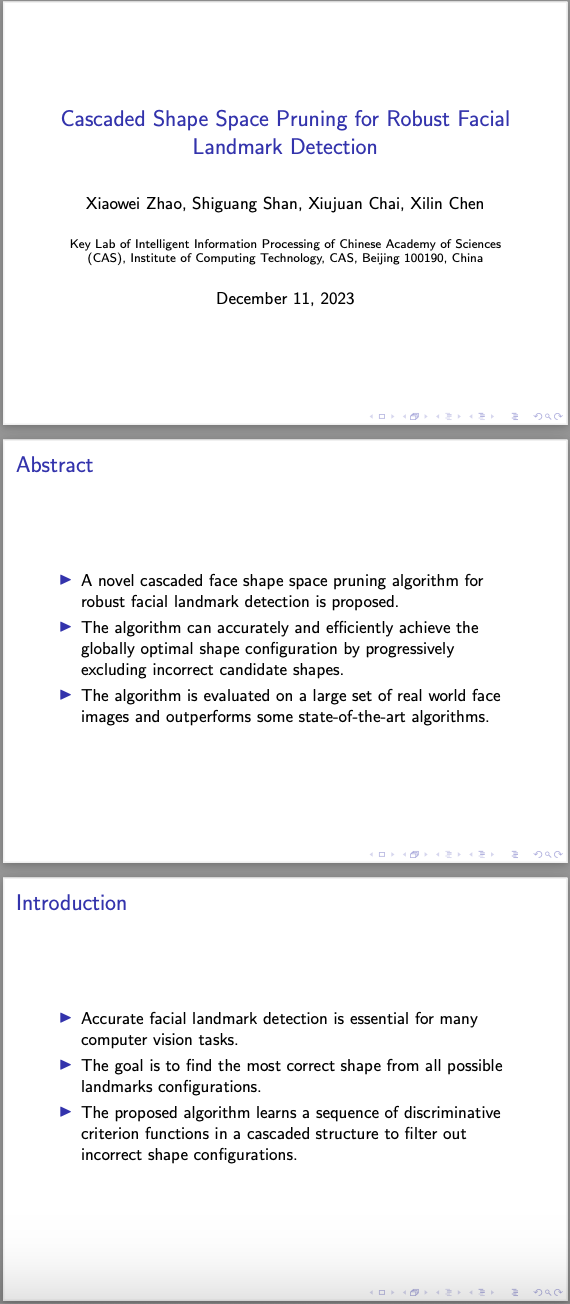
\includegraphics[width=.95\textwidth]{research-chapters/3-chapter/images/ex-poster-skiprep.png}}
        \caption{Document generated without the intermediate representation. This example is cropped for space and includes an additional 3 slides.}
    \end{subfigure}%
    ~ 
    \begin{subfigure}[t]{0.45\textwidth}
        \centering
        \frame{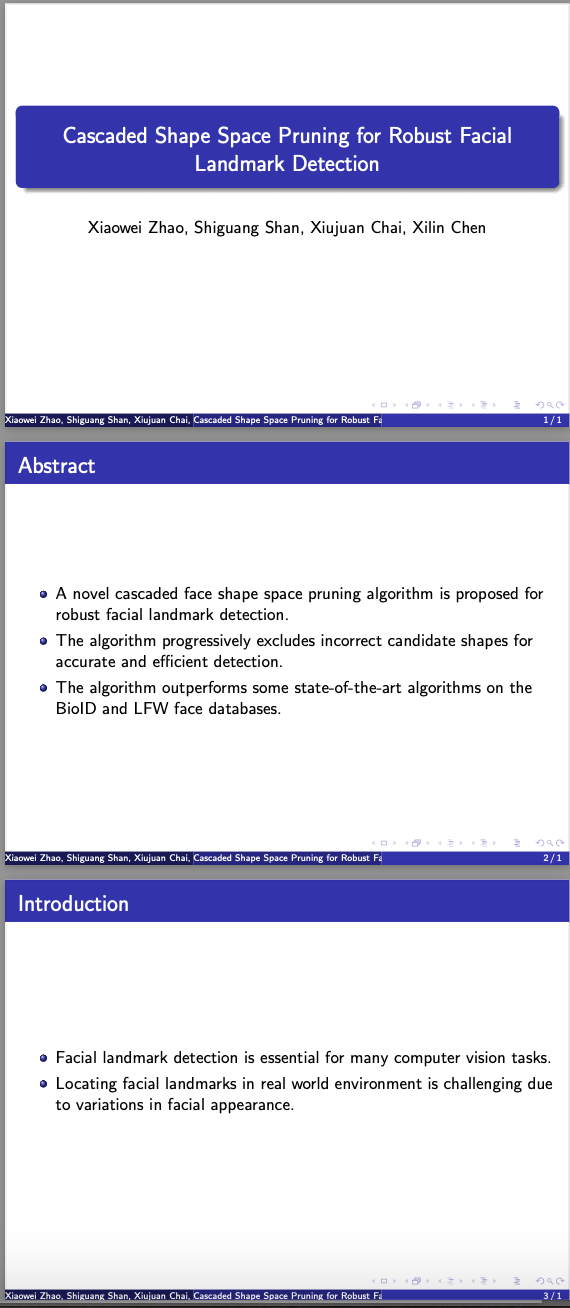
\includegraphics[width=.95\textwidth]{research-chapters/3-chapter/images/ex-poster-withrep.png}}
        \caption{Document generated with the intermediate representation. This example is cropped for space and includes an additional 4 slides.}
    \end{subfigure}
    \caption{The above documents are example posters generated by GPT4 ($\texttt{gpt4-32k}$) with and without the intermediate representation. We found that GPT4 often generates slide decks in place of posters. We can see that the document generated without the intermediate representation contains more verbose panels and includes less formatting.}
    \label{fig:ex-posters}
\end{figure*}